\problemname{Mineraalilademed}

\illustration{.3}{img/turnbull.jpg}{Muda koorub ja paljastab uusi mineraale. Foto: Michael D.\ Turnbull, litsents: CC BY-SA.}

\noindent
Sa töötad maavälises kaevandusfirmas signaalitöötluse kallal. Hetkel on sinu tähelaev asteroidile lähenemas.
Esialgsete seireandmete alusel on põhjust arvata, et asteroidil on $k$~mineraalilademet. Nende täpsed asukohad on aga teadmata.

\medskip

Kirjeldame asteroidi pinda kui täisarvuliste koordinaatidega ruudustikku.
$i$-s mineraalilade asub teadmata positsioonil $(x_i, y_i)$, kus
$-b \le x_i \le b$ and $-b\le y_i \le b$. %constraint:depositcoords
Siin $b$ on mingi täisarv, mis vastab esialgse seire ulatusalale.

Mineraalilademete täpsete asukohtade leidmiseks saad sa saata asteroidi pinnale sonde.
Sondid saadetakse lainete kaupa, mitu sondi korraga.

Oletame, et saatsid $d$~sondist koosneva laine asteroidi pinnale, koordinaatidele $(s_j,t_j)$
iga $1 \leq j \leq d$ kohta.
Kui sond jõuab oma asukohale, arvutab see Manhattani kauguse iga $k$~mineraalilademeni ja saadab kaugused tähelaevale tagasi.
Kõik andmepaketid saabuvad samal ajal, seega ei ole võimalik teada saada, millised kaugused on millise sondi saadetud.
Niisiis tagastab laine $k\cdot d$ täisarvulist kaugust:
\[|x_i-s_j| + |y_i - t_j| \qquad\text{iga } i \in \{1,\ldots,k\} \text{ ja } j \in\{ 1,\ldots,d\} \text{ kohta}\,.\]

Sinu ülesanne on minimeerida pinnale saadetud sondide arv.

\section*{Interaktsioon}

See on interaktiivne ülesanne.
Interaktsioon algab, kui sa loed sisendist ühe rea, mis koosneb kolmest täisarvust $b$, $k$ ja $w$:
ruudustiku piir~$b$,
mineraalilademete arv~$k$,
maksimaalne lainete arv~$w$, mida sul on lubatud saata.

Seejärel saad sa küsida ülimalt $w$ päringut, millest igaüks vastab ühele lainele.
Päring koosneb sümbolist \texttt{?}, millele järgnevad $2d$ tühikutega eraldatud täisarvu:
``\texttt{?} $s_1$ $t_1$ $\cdots$ $s_d$ $t_d$'', kus laines olevate sondide arv~$d$ peab rahuldama
tingimust $1\leq d\leq 2000$. % constraint:wavesize
Väärtused $(s_i, t_i)$ tähistavad $i$-nda sondi koordinaate ja peavad rahuldama tingimusi
$-10^8 \leq s_i \leq 10^8$ ja $-10^8 \leq t_i \leq 10^8$. % constraint:probecoordinates
Vastuseks tuleb üks rida, mis koosneb mittekahanevas järjekorras $k \cdot d$ täisarvust:
kõikide mineraalilademete ja sondikoordinaatide paaride vahelised Manhattani kaugused.
Sondide koguarv üle kõikide lainete ei tohi ületada
$2\cdot 10^4.$ % constraint:totalprobes

Interaktsioon lõpeb, kui trükid välja ühe rea, mis koosneb sümbolist \texttt{!}, millele järgnevad $k$ tühikutega eraldatud arvu $x_1, y_1, x_2, y_2, \ldots, x_k, y_k$.
See peab olema viimane sinu poolt trükitud väljundirida.

Vastus loetakse korrektseks, kui trükid välja kõikide mineraalilademete asukohad.
Need võid välja trükkida mistahes järjekorras.

\section*{Piirangud ja hindamine}

Alati kehtivad
$1\leq b \leq 10^8$, % constraint:b
$1 \leq k \leq 20$, % constraint:k
ja
$2 \le w \le 10^4$. % constraint:w

Selles ülesandes on testid jagatud gruppidesse, iga grupp on väärt mingi arvu punkte.
Iga grupi eest saavad punkte vaid need lahendused, mis läbivad kõik sellesse gruppi kuuluvad testid.
Sinu lõplik skoor on esituste maksimum.

\medskip
\begin{tabular}{lll}
Grupp & Punktid & Lisapiirangud \\\hline
  $1$ & $16$ & $k = 1, w = 10^4$\\
  $2$ & $19$ & $w \ge 500$\\
  $3$ & $11$ & $w \ge 210$\\
  $4$ & $13$ & $w \ge 130$\\
  $5$ & $14$ & $w \ge 3$, $b \le 10^4$\\
  $6$ & $14$ & $w \ge 3$, $b \le 10^7$\\
  $7$ & $13$ & \emph{Lisapiirangud puuduvad}
\end{tabular}

\section*{Example}

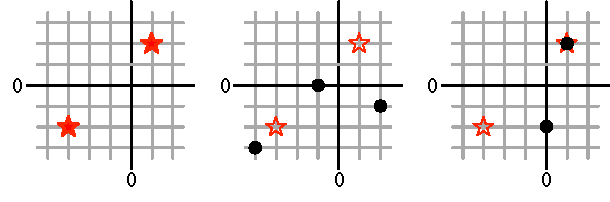
\includegraphics[width=.6\textwidth]{img/sample1.pdf}

Selles näites on $k=2$ mineraaliladet, mis asuvad positsioonidel $(1,2)$ ja $(-3,-2)$. Need on kujutatud punaste tähekestena.
Esimese lainega võid saata näiteks $d=3$ sondi koordinaatidele $(-4,-3)$, $(-1, 0)$ ja $(2,-1)$, mida on kujutatud mustade täppidena.
See laine tagastab $6$ kaugust \[
  2, 4, 4, 4, 6, 10\,.
\]
Järgmise lainega võid saata näiteks $d=2$ sondi koordinaatidele $(1,2)$ ja $(0,-2)$.
See laine tagastab $4$ kaugust \[
  0, 3, 5, 8\,.
\]
